\documentclass[compress]{beamer}
\usepackage{ifthen,verbatim}

\newcommand{\isnote}{}
\xdefinecolor{lightyellow}{rgb}{1.,1.,0.25}
\xdefinecolor{darkblue}{rgb}{0.1,0.1,0.7}

%% Uncomment this to get annotations
%% \def\notes{\addtocounter{page}{-1}
%%            \renewcommand{\isnote}{*}
%% 	   \beamertemplateshadingbackground{lightyellow}{white}
%%            \begin{frame}
%%            \frametitle{Notes for the previous page (page \insertpagenumber)}
%%            \itemize}
%% \def\endnotes{\enditemize
%% 	      \end{frame}
%%               \beamertemplateshadingbackground{white}{white}
%%               \renewcommand{\isnote}{}}

%% Uncomment this to not get annotations
\def\notes{\comment}
\def\endnotes{\endcomment}

\setbeamertemplate{navigation symbols}{}
\setbeamertemplate{headline}{\mbox{ } \hfill
\begin{minipage}{5.5 cm}
\vspace{-0.75 cm} \small
\end{minipage} \hfill
\begin{minipage}{4.5 cm}
\vspace{-0.75 cm} \small
\begin{flushright}
\ifthenelse{\equal{\insertpagenumber}{1}}{}{Muon Alignment News \hspace{0.2 cm} \insertpagenumber\isnote/\pageref{numpages}}
\end{flushright}
\end{minipage}\mbox{\hspace{0.2 cm}}\includegraphics[height=1 cm]{../cmslogo} \hspace{0.01 cm} \vspace{-1.05 cm}}

\begin{document}
\begin{frame}
\vfill
\begin{center}
\textcolor{darkblue}{\Large Muon Alignment News}

\vfill
\begin{columns}
\column{0.75\linewidth}
\begin{center}
\large
{\it Jim Pivarski} \hspace{0.5 cm} Gervasio Gomez
\end{center}
\end{columns}

\vfill
 2 July, 2010

\end{center}
\end{frame}

%% \begin{notes}
%% \item This is the annotated version of my talk.
%% \item If you want the version that I am presenting, download the one
%% labeled ``slides'' on Indico (or just ignore these yellow pages).
%% \item The annotated version is provided for extra detail and a written
%% record of comments that I intend to make orally.
%% \item Yellow notes refer to the content on the {\it previous} page.
%% \item All other slides are identical for the two versions.
%% \end{notes}

\small

\begin{frame}
\frametitle{Organization}
\begin{itemize}\setlength{\itemsep}{0.75 cm}
\item Gervasio and I have been nominated as co-conveners of the \\ Muon Alignment Group

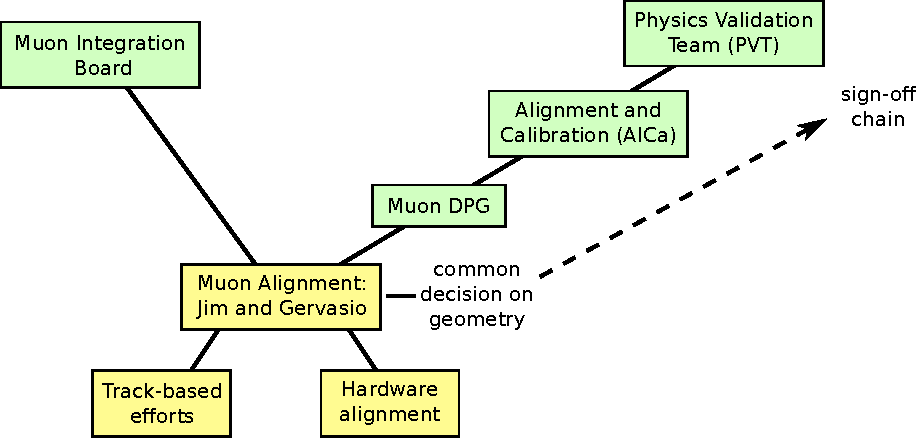
\includegraphics[width=\linewidth]{organization.pdf}

\item The sign-off chain is formalized, but long: we'll need to have a
  common decision on a muon geometry within the group a few weeks in
  advance of the CMS-wide sign-off
\end{itemize}
%% \hspace{-0.83 cm} \textcolor{darkblue}{\Large Outline2}
\end{frame}

\begin{frame}
\frametitle{Quasi-static alignment}
\begin{itemize}
\item Even when a requested sign-off date is announced in advance, slippage
  can make the actual date uncertain

\item To avoid being caught without an agreed-upon geometry, we should
  always have a ``state-of-the-art'' on hand

\vspace{0.2 cm}
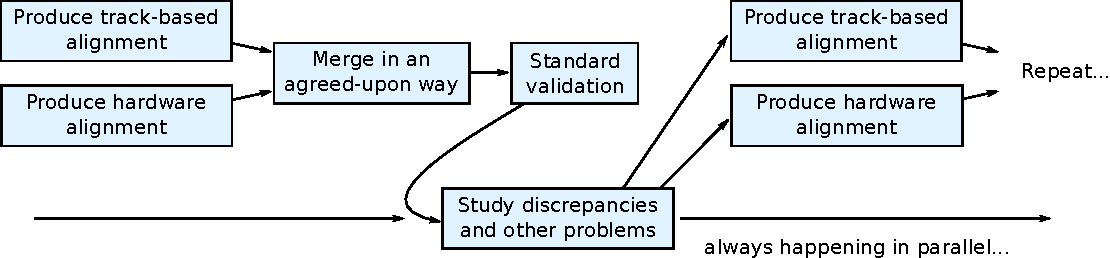
\includegraphics[width=\linewidth]{quasistatic.pdf}

\item The discrepancies/problems that we're working on are usually
  motivated by the results of validation anyway: having a validated
  working point formalizes that (and can help assess priorities)
\end{itemize}
\end{frame}

\begin{frame}
\frametitle{Today's agenda}
\begin{itemize}
\item Major topic: relative track-based/hardware ``barrel twist''

\begin{itemize}
\item largest/most systematic track-based-vs-hardware difference
\item goal: to express what was actually measured very clearly, to figure out where to look to resolve the apparent contradiction
\end{itemize}
\end{itemize}

\begin{center}
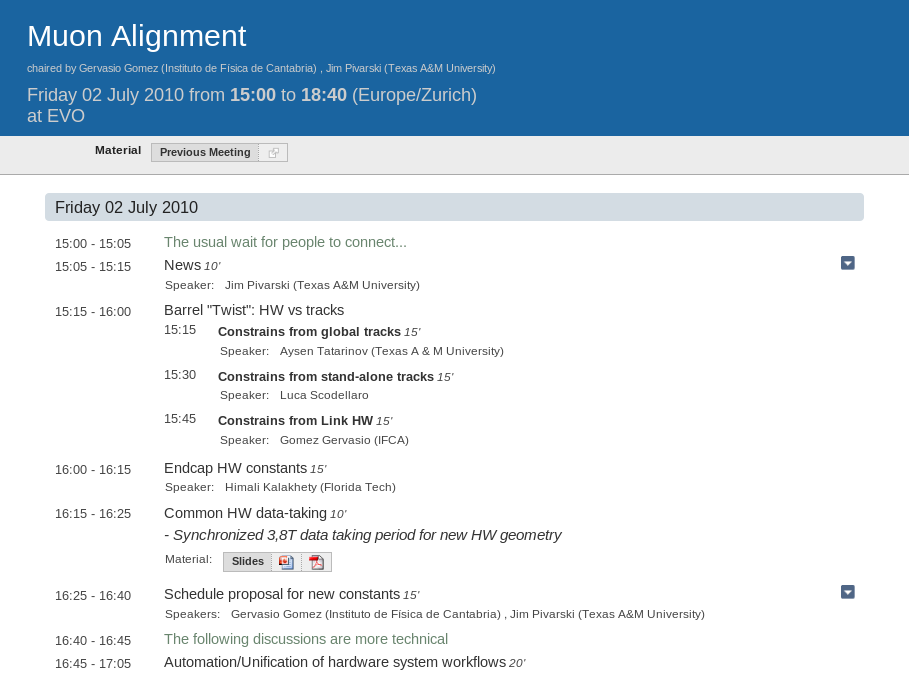
\includegraphics[width=0.75\linewidth]{agenda.png}
\end{center}
\end{frame}

\begin{frame}
\frametitle{Meeting schedule in general}
\begin{description}
\item[Common sessions:] specific details of interest to both groups;
  in particular, comparison/merging of results, what the final results
  mean (uncertainties, correlations, well/poorly determined
  parameters), standardized validation

\textcolor{darkblue}{Beginning of the Friday meeting probably best for everyone}

\textcolor{darkblue}{Should be kept relatively brief (1--2 hours)}

\item[Hardware details:] operations (e.g.\ problems with specific
  sensors), automated workflow, merging endcap/barrel/link results

\item[Track-based details:] book-keeping and other computer issues,
  framework development, in-progress residuals mysteries, etc.
\end{description}

``Details'' can directly follow the common session, but should we
\begin{itemize}
\item alternate by week?  (less frequent ``details'' sessions)
\item split into parallel sessions on Fridays?  (people can't do both)
\item do track-based details on a different day? (need to schedule)
\end{itemize}
\end{frame}

%% \section*{First section}
%% \begin{frame}
%% \begin{center}
%% \Huge \textcolor{blue}{First section}
%% \end{center}
%% \end{frame}

\begin{frame}
\frametitle{Concluding remarks}
\begin{itemize}
\item I'm looking forward to working with Gervasio on a common alignment solution

\item I'm sure that we can start fresh and come to a good understanding of the muon alignment geometry
\end{itemize}
\label{numpages}
\end{frame}

\end{document}
